\chapter{计算CTL下的遗忘:基于归结的方法}\label{chapter04}
{\em 
已有结果显示,任意的$\CTL$公式可以转换为$\CTLsnf$子句的集合。归结是一种以子句为计算对象的判断可满足性的方法,本章提出一种基于归结的计算遗忘理论的方法。
其主要思想是:首先将给定的$\CTL$公式转换为$\CTLsnf$子句的集合,其次在相应的原子命题上使用归结规则得到归结结果,最后“消除”之前引入的索引和$\start$,最终得到遗忘的结果。其主要流程图如图~\ref{Fig:chapter05:v1uv2}所示。
正如本章所要说明的那样,$\CTL$不具有均匀插值这一属性,基于归结的方法在有的情况下是不能计算出遗忘结果的。然而,在有些$\CTL$子类下,本章提出的方法能够计算出其遗忘结果。}
\begin{figure*}[!htb]
	\centering
	% Requires \usepackage{graphicx}
	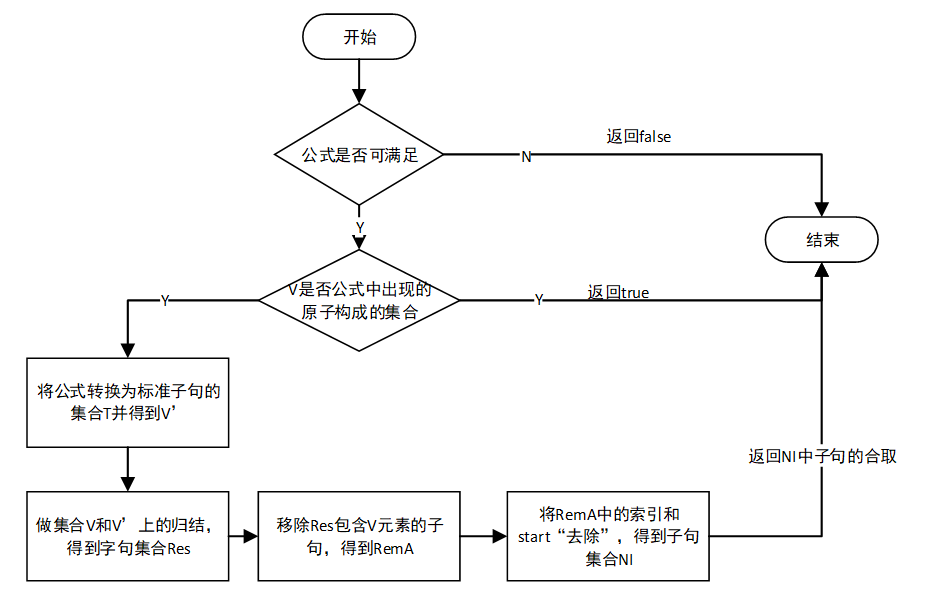
\includegraphics[width=15cm]{chapter04/frame.png}\\
	\caption{基于归结的遗忘的主要流程图}
	\label{Fig:chapter05:v1uv2}
\end{figure*}

\section{引言}
虽然在第\ref{chapter02}章详细介绍了命题逻辑和模态逻辑S5下的基于归结的计算遗忘的方法,但是值得注意的是$\CTL$公式没有像这两种逻辑一样有标准的自身语言子句形式,而$\CTL$的子句是有索引的。这就注定了$\CTL$下的基于归结的遗忘与上述两者的不同,而且也应该要复杂一些(虽有不同,但也可以借鉴)。
本章展示如何使用第~\ref{chapter02:CTLres}节中表~\ref{tab:res}中的归结规则来计算$\CTL$下的遗忘理论。
在本章给定如下约定的记号。令$V\subseteq \Ha$是要遗忘的原子命题的集合,$I\subseteq \Ind$是索引的集合,$V'$表示计算过程所引入的原子命题的集合且满足$V'\cap V=\emptyset$。
此外,$\varphi$是$\CTL$公式,且$T_{\varphi}$是在$\varphi$上使用表~\ref{tab:trans}中的转换规则得到的$\CTLsnf$子句的集合。
显然可以知道,$V'=\Var(T_{\varphi})-\Var(\varphi)$。
在不另加说明的情况下$\Hm$表示五元组$(S,R,L,[\_],s_0)$。
此时,本章所设计的算法的伪代码如算法~\ref{alg:compute:forgetting:by:Resolution}所示。

\begin{algorithm}[htbp]
	\small
	\setstretch{1.2}
	\caption{\emph{ERes}$(\varphi, V)$}
	\label{alg:compute:forgetting:by:Resolution}
	\begin{algorithmic}[1]
		\REQUIRE ~~\\
		\begin{tabular}[t]{p{8mm}l}
			$\varphi$&:$\CTL$公式\\
			$V$&:需要遗忘的原子命题的集合
		\end{tabular}
		\ENSURE ~~\\
		\begin{tabular}[t]{p{8mm}l}
			$ERes(\varphi, V)$&\qquad:公式的合取
			%$SD$&:鞍点策略的支付量
		\end{tabular}
		\IF{$\varphi$ 是不可满足的}
		\RETURN $\bot$;
		\ENDIF
		\IF{$V=\Var(\varphi)$}
		\RETURN $\bot$;
		\ENDIF
		\STATE $T_{\varphi}, V', I \lto \emph{Transform}(\varphi)$;
		\STATE $Res \lto \emph{Resolution}(T_{\varphi}, V\cup V')$;
		\STATE $\emph{RemA} \lto \emph{Removing\_atoms}(Res, V)$;
		\STATE $\NI \lto \emph{Removing\_index}(\emph{RemA})$;
		\RETURN $\bigwedge_{\psi \in \NI_{\CTL}} \psi$;
	\end{algorithmic}
\end{algorithm}


算法~\ref{alg:compute:forgetting:by:Resolution}对于输入$\varphi$和$V$,输出结果记为$ERes(\varphi, V)$。
为了实现这一目标,需要解决如下两个主要问题:
\begin{itemize}
	\item[(1)] 如何表示$\CTL$公式和带索引的$\CTL$公式之间的关系?如在第三章中所展示的那样,将一个$\CTL$公式转换为$\CTLsnf$子句的集合会引入新的原子命题和索引。虽然已有的研究说明了$\CTL$公式可以转换为带索引的公式的集合并保证其可满足性,然而并没有表明这两种形式的公式之间的模型具有怎样的联系。本章给出一种扩展的互模拟定义,以描述两种公式的模型之间的关系。
	\item[(2)] 如何“移除”无关的原子命题(包括需要遗忘的原子命题和转换过程中引入的新的原子命题),以及如何“消除”索引?为此,本章给出“移除”原子命题的一般操作,对应算法~\ref{alg:compute:forgetting:by:Resolution}中的$\emph{Removing\_atoms}(Res, V)$过程,并提出一种一般化的Ackermann引理。为了“消除”索引,探索几个几个逻辑等价关系,对应算法~\ref{alg:compute:forgetting:by:Resolution}中的$\emph{Removing\_index}(\emph{RemA})$过程。
\end{itemize}

本章其余部分组织如下:首先,第\ref{chapter4:sub:biVB}节给出二元互模拟的定义及其相关性质。其次,第\label{chp4:sect:res}节从分节详细地介绍算法~\ref{alg:compute:forgetting:by:Resolution}如何使用基于归结的方法计算遗忘。第三,第~\ref{chp4:sect:complex}节分析算法~\ref{alg:compute:forgetting:by:Resolution}的可终止性及其时间和空间复杂性。最后总结本章的主要工作。



\section{二元互模拟}
\label{chapter4:sub:biVB}
对于给定的初始$\Ind$-结构,这里定义一种$\tuple{V, I}$-互模拟关系。为了与一元的(只考虑原子命题的集合)$V$-互模拟对应,称$\tuple{V, I}$-互模拟为二元互模拟。其在$V$-互模拟的基础上又考虑了索引的集合在结构间关系。
\begin{definition}[二元互模拟] \label{def:VInd:bisimulation}
	令$V\subseteq \Ha$、$I\subseteq \Ind$分别是原子命题和索引的集合,${\cal K}_i=(\Hm_i,s^i)$是初始$\Ind$-结构,其中$\Hm_i=(S_i, R_i, L_i, [\_],s_0^i)$ $(i=1,2)$。称${\cal K}_1$和${\cal K}_2$是 $\tuple{V, I}$-互模拟的(记为${\cal K}_1 \lrto_{\tuple{V, I}} {\cal K}_2$),当且仅当${\cal K}_1 \lrto_V {\cal K}_2$且$\forall j\in (\Ind - I)$有:
	\begin{itemize}
		\item 对任意的$(s,s_1) \in [j]_1$,存在$(s',s_1')\in [j]_2$使得$s\lrto_V s'$且$s_1 \lrto_V s_1'$;
		\item 对任意的$(s',s_1') \in [j]_2$,存在$(s,s_1)\in [j]_1$使得$s\lrto_V s'$且$s_1 \lrto_V s_1'$。
	\end{itemize}
	
\end{definition}

由定义~\ref{def:VInd:bisimulation}可知,当探讨的公式为$\CTL$公式时,因为不用考虑索引,$\lrto_{\tuple{V, I}}$“降维”为$\lrto_V$。
与$\lrto_V$类似,$\lrto_{\tuple{V, I}}$在本文中至关重要的两个性质如下。
\begin{proposition}\label{pro:VI:div}
	令$V_1,V_2\subseteq \Ha$为原子命题的集合,$I_1, I_2 \subseteq \Ind$为索引的集合,${\cal K}_i = (\Hm_i, s_0^i)$ $(i=1,2,3)$为初始$\Ind$-结构。若${\cal K}_1 \lrto_{\tuple{V_1,I_1}} {\cal K}_2$、${\cal K}_2 \lrto_{\tuple{V_2,I_2}} {\cal K}_3$,则:
	\begin{itemize}
		\item[(i)] ${\cal K}_1 \lrto_{\tuple{V_1\cup V_2,I_1\cup I_2}} {\cal K}_3$;
		\item[(ii)] 如果$V_1 \subseteq V_2$且$I_1 \subseteq I_2$,则${\cal K}_1 \lrto_{\tuple{V_2,I_2}} {\cal K}_2$。
	\end{itemize}
\end{proposition}
\begin{proof}
	(i) 由定义~\ref{def:VInd:bisimulation}可知${\cal K}_1 \lrto_{V_1} {\cal K}_2$、${\cal K}_2 \lrto_{V_2} {\cal K}_3$,因此由命题~\ref{pro:div}可知${\cal K}_1 \lrto_{V_1\cup V_2} {\cal K}_3$。
	
	${\cal K}_1 \lrto_{\tuple{V_1,I_1}} {\cal K}_2$\\
	$\Rto$ $\forall j\in (\Ind-(I_1\cup I_2))$有:$\forall(s,s_1) \in [j]_1$,$\exists (s', s_1')\in [j]_2$使得$s\lrto_{V_1} s'$,$s_1\lrto_{V_1} s_1'$\\
	$\Rto$ 又因为${\cal K}_2 \lrto_{\tuple{V_2,I_2}} {\cal K}_3$,所以$\exists (s'', s_1'')\in [j]_3$使得$s'\lrto_{V_2} s''$,$s_1'\lrto_{V_2} s_1''$  \hfill \\
	$\Rto$ $s \lrto_{V_1\cup V_2} s''$且$s_1 \lrto_{V_1\cup V_2} s_1''$
	
	同理可证,$\forall (s'',s_1'')\in [j]_3$,$\exists (s,s_1)\in [j]_1$使得$s \lrto_{V_1\cup V_2} s''$且$s_1 \lrto_{V_1\cup V_2} s_1''$。
	因此,由定义~\ref{def:VInd:bisimulation}可知${\cal K}_1 \lrto_{\tuple{V_1\cup V_2,I_1\cup I_2}} {\cal K}_3$。
	
	(ii)可以由命题~\ref{pro:div}中的(ii)可得。
\end{proof}

对于给定的$\Ind$-Kripke结构$\Hm=(S,R,L,[\_],s_0)$和$\Hm'=(S',R',L',[\_],s_0')$,$\Hm$和$\Hm'$之间的二元互模拟关系$\lrto_{\tuple{V,I}}$给描述公式间在二元组$\tuple{V,I}$上的等价关系提供了前提条件。这同时也为解决本章引言部分提出的问题$(1)$奠定了基础。

\begin{definition}
	给定两个公式(或公式的集合)$T_1$和$T_2$,$I\subseteq \Ind$是索引的集合,$V''\subseteq \Ha$是原子命题的集合。如果下面条件被满足,则称$T_1$和$T_2$在二元组$\tuple{V,I}$上逻辑等价(记为$T_1\equiv_{\tuple{V,I}} T_2$):
	\begin{itemize}
		\item $\forall (\Hm,s_0)\in \Mod(T_1)$,$\exists (\Hm',s_0')\in \Mod(T_2)$使得$(\Hm,s_0) \lrto_{\tuple{V, I}} (\Hm',s_0')$,且
		\item $\forall (\Hm',s_0')\in \Mod(T_2)$,$\exists (\Hm,s_0)\in \Mod(T_1)$使得$(\Hm,s_0) \lrto_{\tuple{V, I}} (\Hm',s_0')$。
	\end{itemize}
	
\end{definition}



\section{基于归结的方法计算遗忘}
\label{chp4:sect:resf}
在本节中,将围绕之前提出的两个问题和算法~\ref{alg:compute:forgetting:by:Resolution}中的几个关键步骤(第7到第11行)来证明$ERes(\varphi, V) \equiv_{\tuple{V',\emptyset}} \CTLforget(\varphi, V)$。在这个等价关系中$\varphi$为$\CTL$公式,$V$为需要遗忘的原子命题的集合,$V'$是将$\varphi$转换为$\CTLsnf$子句集合过程中引入的新的原子命题的集合。这个结论表明,如果$ERes(\varphi, V)$公式中不包含$V'$中的元素,或者$\IR(ERes(\varphi, V), V')$,则$ERes(\varphi, V)$就是从$\varphi$中遗忘掉$V$中的原子命题之后得到的结果。

\subsection{将$\CTL$公式转换为$\CTLsnf$子句的集合}
将$\CTL$公式$\varphi$转换为$\CTLsnf$子句的集合这一过程(记为$Trangsform(\varphi)$)对应算法~\ref{alg:compute:forgetting:by:Resolution}中的第7行所代表的过程。
对于输入$\varphi$,该过程事先将$\varphi$转换为其否定范式(记为$\nnf(\varphi)$),然后通过下面的等价关系\cite{zhang2014resolution,DBLP:books/el/leeuwen90/Emerson90}将出现在公式中的$\top$和$\bot$“去掉”(记为$\simp(\nnf(\varphi))$)。
\begin{align*}
	& (\varphi \wedge \top) \equiv \varphi && (\varphi \wedge \bot) \equiv \bot && (\varphi \vee \top)\equiv \top && (\varphi \vee \bot) \equiv \varphi \\
	& \neg \top \equiv \bot && \neg \bot \equiv \top && QT \bot \equiv \bot && QT \top \equiv \top  \\
	& Q(\varphi \UNTILL \bot) \equiv \bot  && Q(\varphi \UNTILL \top) \equiv \top && Q(\bot \UNTILL \varphi) \equiv \varphi && Q(\top \UNTILL \varphi) \equiv Q\FUTURE \varphi\\
	& Q(\varphi \UNLESS \bot) \equiv Q \GLOBAL \varphi  && Q(\varphi \UNLESS \top) \equiv \top && Q(\bot \UNLESS \varphi) \equiv \varphi && Q(\top \UNLESS \varphi) \equiv \top
\end{align*}
在上述等价关系中,$Q\in \{\ALL,\EXIST\}$是路径量词,$T\in \{\FUTURE, \GLOBAL, \NEXT\}$是时序操作符。

在得到$\simp(\nnf(\varphi))$后,将$T_{\varphi}$初始化为$\{\ALL \GLOBAL(\start \rto p), \ALL \GLOBAL(p \rto \simp(\nnf(\varphi)))\}$,然后转换过程从表~\ref{tab:trans}中找到匹配的规则来将$T_{\varphi}$中的非$\CTLsnf$子句形式的公式转换为$\CTLsnf$子句,并将得到的结果更新$T_{\varphi}$直到$T_{\varphi}$中不存在非$\CTLsnf$子句形式的公式。这个转换过程被写为算法~\ref{alg:compute:trans}。


\begin{algorithm}[htbp]
	\small
	\setstretch{1.2}
	\caption{\emph{Transform}$(\varphi)$}
	\label{alg:compute:trans}
	\begin{algorithmic}[1]
		\REQUIRE ~~\\
		\begin{tabular}[t]{p{8mm}l}
			$\varphi$&:$\CTL$公式
		\end{tabular}
		\ENSURE ~~\\
		\begin{tabular}[t]{p{8mm}l}
			$T_{\varphi}$&: $\CTLsnf$子句的集合\\
			$V'$& : 新引入的原子命题的集合\\
			$I$ &: 引入的索引的集合
			%$SD$&:鞍点策略的支付量
		\end{tabular}
		\STATE $T_{\varphi}\lto \{\ALL \GLOBAL(\start \rto p), \ALL \GLOBAL(p \rto \simp(\nnf(\varphi)))\}$;(其中$p\in {\cal A}-var(\varphi)$)
		\STATE $V'\lto \{p\}$;
		\STATE $I\lto \emptyset$;
		\WHILE{$\exists \psi \in T_{\varphi}$使得$\psi$不是$\CTLsnf$子句}
		\STATE $T_{\varphi} \lto T_{\varphi}-\{\psi\}$;
		\STATE $T_{\varphi} \lto Trans(\psi) \cup T_{\varphi}$;
		\IF{$Trans(\psi)$引入了一个新原子命题$q$}
		\STATE $V'\lto V' \cup \{q\}$;
		\ENDIF
		\IF{$Trans(\psi)$引入了一个新的索引$ind$}
		\STATE $I\lto I \cup \{ind\}$;
		\ENDIF
		\ENDWHILE
		\RETURN $T_{\varphi}, V', I$;
	\end{algorithmic}
\end{algorithm}


在算法~\ref{alg:compute:trans}中,$Trans(\psi)$表示使用表~\ref{tab:trans}中的某一条规则来转换$\psi$(规则中长横线上面的部分),并返回规则的结果(规则中长横线下面的部分)、引入的新原子命题和索引。这里使用规则\textbf{Trans(6)}为例来描述这一过程。令$\psi=q \rto \ALL \NEXT \phi$,可以看出当$\phi$不是经典子句的时候$\psi$不是$\CTLsnf$子句,且规则\textbf{Trans(6)}是能使用的(匹配的)规则,则$Trans(\psi)$对$\psi$使用规则\textbf{Trans(6)}并返回结果$\{q \rto \ALL \NEXT q', q' \rto \phi\}$(在这里,引入了新的原子命题$q'$,但是没有引入新的索引)。

\begin{proposition}\label{pro:TranE}
	令$\varphi$是一个$\CTL$公式,$(T_{\varphi}, V', I) = Transform(\varphi)$,则$\varphi \equiv_{\tuple{V',I}} T_{\varphi}$。
\end{proposition}
\begin{proof}
	为了讨论方便,令$Transform(\varphi)$过程产生了一个公式集合的序列,$T_0, T_1, \dots, T_n=T_{\varphi}$,其中$p$是不出现在$\varphi$中的原子命题,$T_0=\{\ALL \GLOBAL(\start \rto p), \ALL \GLOBAL(p \rto \simp(\nnf(\varphi)))\}$且对任意的$i$($0\leq i < n$)有$T_{i+1} = (T_i-\{\psi\}) \cup R_i$($Trans(\psi)$返回的结果为$R_i$)。此外,在这一过程中,所有的公式都是其否定范式的形式。
	
	为了证明命题中的结论成立,只需证明,对任意的$i$($0\leq i < n$)有$T_i \equiv_{\tuple{V',I}} T_{i+1}$成立。由于$T_{i+1}$是由$T_i$通过表~\ref{tab:trans}中的规则作用于$T_i$中的某一个公式得到,因此证明过程分为两个部分:(1)从$\varphi$到$T_0$部分;(2)对表~\ref{tab:trans}中的规则做归纳的部分。为了方便,下面假设$\Hm_1=(S_1,R_1,L_1,[\_],s_1)$和$\Hm_2=(S_2,R_2,L_2, [\_]_2, s_2)$。
	
	(1)这里将证明$\varphi \equiv_{\tuple{\{p\},\emptyset}} T_0$。
	
	$(\Rto)$ $\forall (\Hm_1, s_1) \in \Mod(\varphi)$,可以构造一个$\Ind$-Kripke结构$\Hm_2=(S_2,R_2,L_2,[\_],s_2)$使得$\Hm_2$除了$L_2(s_2)=L_1(s_1) \cup \{p\}$(默认不出现在$\varphi$中的原子命题都不出现在状态的标签中),其他的元素都与$\Hm_1$中元素相同。显然,$(\Hm_2,s_2)\models T_0$且$(\Hm_1,s_1) \lrto_{\tuple{\{p\}, \emptyset}} (\Hm_2, s_2)$。
	
	$(\Lto)$ $\forall (\Hm_1,s_1) \in \Mod(T_0)$,由$\start$的语义可以知道$(\Hm_1,s_1) \models \varphi$。
	
	(2)这里将证明对任意的$i$($0\leq i < n$)有$T_i \equiv_{\tuple{V',I}} T_{i+1}$成立,其中$T_{i+1} = (T_i-\{\psi\}) \cup R_i$。为了方便,用$\psi \rto_t R_i$表示$R_i$是使用规则$t$在公式$\psi$上得到的结果,且$T_i=X\cup \{\psi\}$(显然,$T_{i+1}=X\cup R_i$)。下面证明规则$t\in \{$\textbf{Trans(1), Trans(4), Trans(6)}$\}$的情形,其他情形可以类似地证明。
	
	(a)$t=\textbf{Trans(1)}$。
	
	$(\Rto)$ $\forall (\Hm_1,s_1)\in \Mod(T_i)$,即$(\Hm_1, s_1) \models X \wedge \ALL\GLOBAL(q \rto \EXIST \NEXT \varphi)$\\
	$\Rto$ $(\Hm_1,s_1) \models X$,且对任意路径$\pi$上的状态$s_{1,j}$ $(j\geq 1)$有:$(\Hm,s_{1,j}) \not \models \neg q$或存在一个状态$s_{1,j+1}$使得$(s_{1,j},s_{1,j+1})
	 \in R_1$且$(\Hm,s_{1,j+1}) \models \varphi$。
	
	由此可以构造一个$\Ind$-Kripke结构$\Hm_2$使得$\Hm_2$与$\Hm_1$相同,除了对使用规则$\textbf{Trans(1)}$在公式$\ALL\GLOBAL(q \rto \EXIST \NEXT \varphi)$上而引入的新索引$ind$有$[ind]_2=\bigcup_{s\in S} R_s \cup R_y$。其中:
	\begin{itemize}
		\item $R_{s_{1,j}}=\{(s_{1,j}, s_{1,j+1}), (s_{1,j+1}, s_{1,j+2}),\dots\}$ $(j\geq 1)$,其满足“若$(\Hm_1,s_{1,j}) \models q$,则$(\Hm_1,s_{1,j+1})$ $\models \varphi$”且“对于任意的$i\geq j$,若$(s_{1,i}, s') \in R_s\ (s \not= s_{1,j})$,则$s'=s_{1,i+1}$”;
		\item $R_y=\{(s_x,s_y)\mid s_x\in S$,若$\forall(s_1',s_2') \in \bigcup_{s\in S} R_s$, $s_1'\not= s_x$,则找一个状态$s_y\in S_2$使得$(s_x,s_y)\in R_2\}$。
	\end{itemize}

显然,$(\Hm_1,s_1) \lrto_{\tuple{\emptyset,\{ind\}}} (\Hm_2,s_2)$\\
$\Rto$ 对任意从$s_2$开始的路径$\pi=( s_2= s_{2,1} , s_{2,2}, \dots)$,如果$s_{2,j} \in \pi$,则$(\Hm_2,s_{2,j}) \models \neg q$或者$(\Hm_2,s_{2,j}) \models \EXIST_{\tuple{ind}} \NEXT \varphi$\\
$\Rto$ $(\Hm_2,s_2)\models \ALL\GLOBAL(q \rto \EXIST_{\tuple{ind}} \NEXT \varphi)$\\
$\Rto$ $(\Hm_2,s_1) \models X \wedge \ALL\GLOBAL(q \rto \EXIST_{\tuple{ind}} \NEXT \varphi)$

$(\Lto)$ $\forall (\Hm_1,s_1) \in \Mod(T_{i+1})$,即$(\Hm_1,s_1) \models X \wedge \ALL \GLOBAL(q \rto \EXIST_{\tuple{ind}} \NEXT \varphi )$\\
$\Rto$ $(\Hm_1,s_1) \models X$且$(\Hm_1,s_1) \models \ALL \GLOBAL(q \rto \EXIST_{\tuple{ind}} \NEXT \varphi)$\\
$\Rto$ 对任意的以$s_1$为始点的路径上的任意状态$s_{1,j}$,$(\Hm_1,s_{1,j}) \models \neg q$或$(\Hm_1,s_{1,j}) \models \EXIST\NEXT\varphi$\\
$\Rto$ $(\Hm_1,s_1) \models \ALL\GLOBAL(q \rto \EXIST \NEXT \varphi)$\\
$\Rto$ $(\Hm_1,s_1) \models X \wedge \ALL\GLOBAL(q \rto \EXIST \NEXT \varphi)$。

	(b)$t=\textbf{Trans(4)}$。
	
   $(\Rto)$	$\forall(\Hm_1,s_1) \in \Mod(T_i)$,即$(\Hm_1,s_1) \models X \wedge \ALL\GLOBAL (q \rto \varphi_1 \vee \varphi_2)$ \\
   $\Rto$ $(\Hm_1,s_1) \models X$且$\forall s_1'\in S_1$,$(\Hm_1, s_1') \models q \rto \varphi_1 \vee \varphi_2$\\
   $\Rto$ $(\Hm_1,s_1')\models \neg q$或$(\Hm_1,s_1')\models \varphi_1 \vee \varphi_2$。
   
   可以如下构造$\Ind$-Kripke结构$\Hm_2$:
   \begin{itemize}
   	\item $S_2=S_1$,$R_2=R_1$,$[\_]_2$与$[\_]_1$一样且$s_2=s_1$;
   	\item $L_2$与$L_1$类似,除了:若$(\Hm_1, s_1') \models \neg q$则$L_2(s_1') = L_1(s_1')$,否则“若$(\Hm_1,s_1') \models \varphi_1$ 则 $L_2(s_1')=L_1(s_1')$,否则$L_2(s_1')=L_1(s_1') \cup \{p\}$”。
   \end{itemize}
   显然,$(\Hm_2,s_1') \models (q\rto \varphi_1 \vee p) \wedge (p \rto \varphi_2)$且$(\Hm_1, s_1) \lrto_{\tuple{\{p\}, {\O}}} (\Hm_2, s_2)$, 因而$(\Hm_2,s_1) \models T_{i+1}$。
	
	$(\Lto)$  $\forall (\Hm_1, s_1) \in \Mod(T_{i+1})$,即$(\Hm_1,s_1) \models X \wedge \ALL\GLOBAL (q\rto \varphi_1 \vee p) \wedge \ALL\GLOBAL(p \rto \varphi_2)$。 显然,$(\Hm_1, s_1) \models T_i$。
	
	(c)$t$=\textbf{Trans(6)}。
	
	这里证明$\EXIST_{\tuple{ind}} \NEXT$的情形,$\ALL \NEXT$情形可以类似地证明。
	
	$(\Rto)$ $\forall(\Hm_1,s_1) \in \Mod(T_i)$,即$(\Hm_1,s_1) \models X \wedge \ALL\GLOBAL(q \rto \EXIST_{\tuple{ind}}\NEXT \varphi)$\\
	$\Rto$ $(\Hm_1,s_1) \models X$且对任意的$s_1'\in S, (\Hm_1,s_1') \models q \rto \EXIST_{\tuple{ind}} \NEXT \varphi$\\
	$\Rto$ $(\Hm_1,s_1') \models \neg q$或者存在一个状态$s'$使得$(s_1', s') \in [ind]$且$(\Hm_1,s') \models \varphi$\\
	
	可以如下构造$\Ind$-Kripke结构$\Hm_2$:
	\begin{itemize}
		\item $S_2=S_1$,$R_2=R_1$,$[\_]_2$与$[\_]_1$一样且$s_2=s_1$;
		\item $L_2$与$L_1$类似,除了:若$(\Hm_1, s_1') \models \neg q$则$L_2(s_1') = L_1(s_1')$,否则“若$(\Hm_1,s_1') \models q$则$L_2(s')$ $=L_1(s')\cup \{p\}$ $((s_1',s')\in R_2)$”。
	\end{itemize}
	显然,$(\Hm_2,s_2) \models \ALL\GLOBAL(q\rto \EXIST_{\tuple{ind}} \NEXT p) \wedge \ALL\GLOBAL(p \rto \varphi)$, $(\Hm_2,s_2) \models T_{i+1}$且$(\Hm_1, s_1) \lrto_{\tuple{\{p\}, {\O}}} (\Hm_2, s_2)$ ($s_2=s_1$)。
	
	$(\Lto)$ $\forall(\Hm_1, s_1) \in \Mod(T_{i+1})$,即$(\Hm_1,s_1) \models X \wedge \ALL\GLOBAL(q\rto \EXIST_{\tuple{ind}} \NEXT p) \wedge \ALL\GLOBAL(p \rto \varphi)$。显然,$(\Hm_1, s_1) \models T_i$。
\end{proof}

命题~\ref{pro:TranE}表示,对于给定的$\CTL$公式$\varphi$,通过上述的转换过程得到的$\CTLsnf$子句的集合$T_{\varphi}$与$\varphi$在二元组$\tuple{V',I}$上逻辑等价。
下面给出本章的运行示例来展示每一个过程。
%令$(T_{\varphi}, V', I) = Transform(\varphi)$,那么

\begin{example}[运行示例]
	\label{examp:Tran}
	给定公式$\varphi=\ALL((p\wedge q) \UNTILL (f\vee m)) \wedge r$和原子命题的集合$V=\{p,r\}$。$(T_{\varphi}, V', I) = Transform(\varphi)$,其中$V'=\{x,y,z,w\}$($w$是与子句$z \rto \ALL \FUTURE x$对应的新引入的原子命题~\footnote{注意:本文中对每个$Q$-某时子句($Q\in \{\EXIST, \ALL\}$)都产生一个新的原子变量$w$与之对应。}),$I=\emptyset$且$T_{\varphi}$中的元素如下:\\
	$
	\begin{array}{llll}
		\centering
		1. \start\rto z & 2. \top \rto \neg z \vee r \qquad & 3.\top \rto \neg x\vee f \vee m  & 4. \top \rto \neg z \vee x \vee y \\
		5.\top \rto \neg y \vee p &  6.\top \rto \neg y \vee q &
		7. z \rto \ALL \FUTURE x & 8. y \rto \ALL \NEXT(x\vee y).\\
	\end{array}
	$
\end{example}



\subsection{归结过程}
本节的归结过程在转换过程之后执行。给定的公式$\varphi$和原子命题的集合$V$,令$(T_{\varphi}, V', I) = Transform(\varphi)$。在$T_{\varphi}$和$V\cup V'$上的归结过程(记为$Resolution(T_{\varphi}, V \cup V')$)产生一个子句集合的序列$T_0=T_{\varphi}, T_1, T_2$, $\dots$, $T_n=Res$并返回$Res$。在这个序列中,对所有的$0\leq i \leq n$都有$T_{i+1}=T_i\cup R_i$($R_i$是由表~\ref{tab:res}中的某条归结规则作用到$T_i$中的某些子句上得到的结果),且在$Res$中不能再由任何的归结规则产生新的子句(或者产生了矛盾,即子句$\start\rto \bot$和子句$\top \rto \bot$,因为在此情况下可以得出$\CTLforget(\varphi, V) \equiv \bot$)。
值得注意的是,在这一过程中产生的$T_i$($0\leq i \leq n$)是$\CTLsnf$子句的集合。

下面的命题表示$T_{\varphi}$与归结过程得到的结果在二元组$\tuple{V\cup V',\emptyset}$上逻辑等价。

\begin{proposition}
	\label{pro:ResE}
	给定公式$\varphi$和原子命题的集合$V$。若$(T_{\varphi}, V', I) = Transform(\varphi)$,则$T_{\varphi} \equiv_{\tuple{V\cup V', \emptyset}} Resolution(T_{\varphi}, V \cup V')$。
\end{proposition}
\begin{proof}
这一结论可以通过证明$T_i \equiv_{\tuple{V\cup V', \emptyset}} T_{i+1}$($0\leq i < n$),其中$T_{i+1}=T_i\cup R_i$。记$\Pi\rto_r R_i$为通过对$\Pi\subseteq T_i$和原子命题$p\in (V\cap \Var(\Pi))$使用表~\ref{tab:res}中的归结规则$r$得到$R_i$。

(1)	这里证明若$r\in \{\textbf{(SRES1)},$ $\dots,$ $\textbf{(SRES8)},$ $(\textbf{RW1}),$ $(\textbf{RW2})\}$,则$T_i \equiv_{\tuple{\{p\}, {\O}}} T_{i+1}$。

一方面可以证明$\Pi\models R_i$,因而$T_{i+1} \models T_i$。另一方面,由于$T_i\subseteq T_{i+1}$,所以$T_{i+1} \models T_i$。显然$T_i \equiv T_{i+1}$,又$\emptyset \subseteq (V\cup V')$且$\emptyset \subseteq \emptyset$,由命题~\ref{pro:VI:div}可知$T_i \equiv_{\tuple{V\cup V', \emptyset}} T_{i+1}$。

(2)这里证明若$r=$\textbf{(ERES1)},则$T_i \equiv_{\tuple{\{l, w_{\neg l}^{\ALL}\}, {\O}}} T_{i+1}$,其中$w_{\neg l}^{\ALL}\in V'$是与子句$Q \rto \ALL \FUTURE \neg l$相关的新的原子命题,$l$是文字(即:$p$或者$\neg p$)。

在文章~\cite{bolotov2000clausal}中已经证明$\Pi \models R_i$,因此有$T_{i+1}=T_i \cup \Lambda_{\neg l}^{\ALL}$,其中$\Lambda_{\neg l}^{\ALL}$是通过使用表~\ref{tab:trans}中的转换规则作用到$R_i$上得到的$\CTLsnf$子句的集合(请查看文章~\cite{zhang2009refined}获取更加详细的描述)。显然,对所有的$(\Hm_1,s_1) \in \Mod(T_i= X \cup \Pi)$都存在一个$(\Hm_2, s_2)\in \Mod(T_{i+1}=T_i \cup \Lambda_{\neg l}^{\ALL})$使得$(\Hm_1, s_1) \lrto_{\tuple{\{p, w_{\neg l}^{\ALL}\}, {\O}}} (\Hm_2, s_2)$,且对任意的$(\Hm_2, s_2)\in \Mod(T_{i+1}=T_i \cup \Lambda_{\neg l}^{\ALL})$也存在一个$(\Hm_1,s_1) \in \Mod(T_i= X \cup \Pi)$使得$(\Hm_1, s_1) \lrto_{\tuple{\{p, w_{\neg l}^{\ALL}\}, {\O}}} (\Hm_2, s_2)$。
又$\{p, w_{\neg l}^{\ALL}\} \subseteq (V\cup V')$且$\emptyset \subseteq \emptyset$,由命题~\ref{pro:VI:div}可知$T_i \equiv_{\tuple{V\cup V', \emptyset}} T_{i+1}$。

当规则为$\textbf{(ERES2)}$时可以类似地证明。
\end{proof}

命题~\ref{pro:ResE}和命题~\ref{pro:TranE}表明$\varphi \equiv_{\tuple{V'', \emptyset}} Resolution(T_{\varphi}, V'')$,即对任意的公式$\psi$,$\IR(\psi, V'')$蕴涵“$\varphi \models \psi$当且仅当$Resolution(T_{\varphi}, V'') \models \psi$”,其中$V''=V\cup V'$。

\begin{example}[例~\ref{examp:Tran}的延续]\label{examp:Res}
	对例~\ref{examp:Tran}中的$T_{\varphi}$和$V\cup V'$使用上述归结过程,除了例~\ref{examp:Tran}中的子句,还得到如下子句:
	% The \textcolor{red}{resolvent} \textcolor{blue}{resolvents} of $T_{\varphi}$ obtained from Example~\ref{examp:Tran} by executing the resolution process on $T_{\varphi}$ and $V\cup V'$ are the following clauses (in addition to the ones in Example~\ref{examp:Tran}):
	\begin{align*}
		&(1)\ \start \rto r && (1,2,\textbf{SRES5})
		&&(2)\ \start \rto x \vee y && (1,4,\textbf{SRES5})\\
		% \end{align*}
		% \begin{align*}
		&(3)\ \top \rto \neg z \vee y \vee f \vee m && (3, 4, \textbf{SRES8})
		&&(4)\ y \rto \ALL\NEXT(f\vee m\vee y) && (3,8, \textbf{SRES6})\\
		&(5)\ \top \rto \neg z \vee x \vee p && (4,5, \textbf{SRES8})
		&&(6)\ \top \rto \neg z \vee x \vee q && (4,6, \textbf{SRES8})\\
		&(7)\ y \rto \ALL\NEXT(x\vee p) && (5, 8, \textbf{SRES6})
		&&(8)\ y \rto \ALL\NEXT(x\vee q) && (6, 8, \textbf{SRES6})\\
		&(9)\ \start \rto f\vee m \vee y && (3,(2), \textbf{SRES5}) 
		% \end{align*}
		% \begin{align*}
		&&(10)\ \start \rto x \vee p && (5,(2),\textbf{SRES5}) \\
		&(11)\ \start \rto x \vee q && (6,(2), \textbf{SRES5})
		&& (12)\ \top \rto p \vee \neg z \vee f \vee m && (5,(3), \textbf{SRES8})\\
		& (13)\ \top \rto q \vee \neg z \vee f \vee m && (6,(3), \textbf{SRES8})
		&&(14)\ y \rto \ALL\NEXT(p \vee f\vee m) && (5, (4), \textbf{SRES6})\\
		&(15)\ y \rto \ALL\NEXT(q \vee f\vee m) && (6, (4), \textbf{SRES6}) 
		%\end{align*}
		%\begin{align*}
		&&(16)\ \start \rto f\vee m \vee p && (5, (9), \textbf{SRES5}) \\
		&(17)\ \start \rto f\vee m \vee q && (6, (9), \textbf{SRES5})
	\end{align*}
\end{example}



\subsection{“移除”过程}
\label{sec:remV}
本节意在“移除”如何将归结过程得到的结果中含有$V$中原子命题的子句,而保证其在二元组$\tuple{V\cup V, I}$上的逻辑等价关系,这一过程对应算法~\ref{alg:compute:forgetting:by:Resolution}中的第9行。
给定$\CTLsnf$子句$C$和原子命题的集合$V$:
\[Removing\_atoms(C, V) \equiv
\left\{
\begin{array}{ll}
	\top, \qquad \hbox{$\Var(C) \cap V \not = \emptyset$;} \\
	C,  \qquad  \hbox{otherwise.}
\end{array}
\right.
\]
此外,对于$\CTLsnf$子句的集合$\Pi$,
\[Removing\_atoms(\Pi, V) = \{Removing\_atoms(r, V) \mid r \in \Pi\}.\]
可以看出,通过这一过程后得到的子句集合里的子句不再包含$V$中的原子命题的集合且与原集合满足下面关系。

\begin{proposition}\label{pro:remove}
	%Let $V''=V \cup V'$, then we have
	对于给定的公式$\varphi$和原子命题的集合,有:
	$$Resolution(T_{\varphi}, V \cup V') \equiv_{\tuple{V \cup V', \emptyset}}   Removing\_atoms(Resolution(T_{\varphi}, V \cup V'), V).$$
\end{proposition}
\begin{proof}
	因为要考虑的索引集合为空集,所以只需证明:
	$$Resolution(T_{\varphi}, V \cup V') \equiv_{V \cup V'}   Removing\_atoms(Resolution(T_{\varphi}, V \cup V'), V)$$
	其中$\equiv_V$与$\equiv_{\tuple{V,I}}$的定义类似,只是不考虑索引部分。
	为了证明这一过程,下面给出两个事实:
	\begin{itemize}
		\item \textbf{(GNA)} 对任意的$p\in \Var(\varphi)$,$p$都不出现在$\CTLsnf$子句的左边;
		\item \textbf{(PI)} 对任意的$p\in V'$,如果$p$出现在$\CTLsnf$子句的左边,那么$p$为负出现,即该子句关于$p$是负的。
	\end{itemize}

不失一般性地,假设$V=\{p\}$,且规定$Res=Resolution(T_{\varphi}, V \cup V')$、$V''=V\cup V'$、$C_i$是经典子句、$l$是$p$或者$\neg p$。
显然,$Res \models \emph{Removing\_atoms}(Res, V)$,这里将证明对任意的${\cal K}=(\Hm, s)$(${\cal K}\in \Mod(\emph{Removing\_atoms}(Res, V))$且$\Hm=(S, R, L, s)$),存在一个初始结构${\cal K}'=(\Hm', s')$使得${\cal K} \lrto_{V''} {\cal K}'$且${\cal K}' \models Res$。 
接下来从两个大点证明这一结论。

(1)假设全局子句$C=\top\rto C_1 \vee l \in Res$,其中$\Var(l)=\{p\}$。
\begin{itemize}
	\item[] (a) 如果不存在子句$C'\in Res$使得$C$和$C'$在$p$上是可归结的~\footnote{如果能在表~\ref{tab:res}中找到一条规则使得子句$C$和$C'$为该规则的横线上面部分,且相应的文字是$p$,则称$C$和$C'$在$p$上是可归结。},这意味着在$Res$中不存在其他非$Pt$-某时子句包含有文字$\neg l$,其中$Pt\in \{\ALL,\EXIST\}$。则有两种情况需要讨论:
	\begin{itemize}
		\item[] (i) $p \not \in \Var(C')$。$\forall {\cal K}=(\Hm, s)\in \Mod(\emph{Removing\_atoms}(Res, V))$可以如下构造$(\Hm',s')$:令$\Hm'= (S, R, L',s)$ (即$s'=s$),其中$L'$与$L$ 一样,除了对于$s_1\in S$,如果$(\Hm, s_1) \not \models C_1 \vee l$则“若$l=p$,则令$L'(s_1) = L(s_1) \cup \{p\}$,否则令$L'(s_1) = L(s_1) - \{p\}$”。
		\item[] (ii) 如果$C'= Q\rto Pt \FUTURE \neg l$。不失一般性地,假设$l=p$且$Q$为文字($Q$为文字的合取的情形可以类似证明)。$\forall {\cal K}=(\Hm, s)\in \Mod(\emph{Removing\_atoms}(Res, V))$,如下构造$(\Hm',s')$:令 $\Hm'=(S', R', L', s')$,其中$S'=S$,$R'=R$,$s'=s$,且$L'=L$,除了$\forall s\in S'$,“如果$Q$为正文字,则令$L'(s) = L(s) - \{Q\}$,且若$(\Hm, s) \not \models C_1$,则$L'(s) = L(s) \cup \{p\}$”,否则令$L'(s) = L(s)$。
	\end{itemize}
	因此,有${\cal K} \lrto_{V''} {\cal K}'$且${\cal K}' \models Res$。
	\item[] (b)	如果存在子句$C'\in Res$使得$C$和$C'$在$p$上是可归结的。
		\begin{itemize}
		\item[] (i) 若$C'= Q\rto Pt \NEXT (C_2 \vee \neg l)$(这里令$Pt=\GLOBAL$,当$Pt = \EXIST$时可以类似地证明),因此有$Q\rto \GLOBAL \NEXT(C_1 \vee C_2) \in Res$。$\forall {\cal K}=(\Hm, s)\in \Mod(\emph{Removing\_atoms}(Res, V))$,如下构造$(\Hm',s')$:令$\Hm'= (S, R, L',s)$(即:$s'=s$),其中$L'$与$L$类似,除了$\forall s_1\in S$,若$(\Hm, s_1) \not \models Q$,则“$\forall (s_1, s_2) \in R$,若“$(\Hm, s_2) \not \models C_1$,则“若$l=p$,则令$L'(s_2) = L(s_2) \cup \{p\}$,否则$L'(s_2) = L(s_2) - \{p\}$””,否则,若$(\Hm, s_2) \models  C_1 \wedge \neg C_2$,则“若$l=p$,则$L'(s_2) = L(s_2) - \{p\}$,否则$L'(s_2) = L(s_2) \cup \{p\}$””;否则若$(\Hm, s_2) \models \neg C_1 \wedge C_2$,则“若$l=p$,则令$L'(s_2) = L(s_2) \cup \{p\}$,否则$L'(s_2) = L(s_2) - \{p\}$”。显然,${\cal K} \lrto_{V''} {\cal K}'$且${\cal K}' \models C' \wedge C$。
		\item[] (ii) 若$C' =  Q\rto Pt \FUTURE \neg l$。不失一般性地,假设$l=p$。由于$C$和$C'$在$p$上可归结,则存在$\CTLsnf$子句集合$\Pi=\{P_1^1 \rto * C_1^1$, \dots, $P_{m_1}^1 \rto * C_{m_1}^1$, $P_1^n \rto * C_1^n$, \dots, $P_{m_n}^1 \rto * C_{m_n}^1 \}$使得$\bigvee_{i=1}^n \bigwedge_{j=1}^{m_i} P_j^i \rto \EXIST \NEXT \EXIST \GLOBAL l$,其中$*$要么为空字符要么为集合$\{\GLOBAL \NEXT, \EXIST_{\tuple{ind}} \NEXT\}$ 中的某个元素。此外,$\neg C_1 \rto l\in \Pi$。因此,通过规则$\textbf{ERES1}$可以得到子句$C''=\top \rto \neg Q \vee \neg p \vee C_1$(对规则$\textbf{ERES2}$类似)。因此,在子句$C$和$C''$上使用规则$\textbf{SRES8}$可得$\top \rto \neg Q \vee C_1$。$\forall {\cal K}=(\Hm, s)\in \Mod(\emph{Removing\_atoms}(Res, V))$,可以如下构造$(\Hm',s')$:令$\Hm'= (S, R, L',s)$(即:$s'=s$),其中$L'$与$L$类似,除了$\forall s_1\in S$,“若$(\Hm, s_1) \models Q$,则令$L'(s_1) = L(s_1) - \{p\}$,否则令$L'(s_1) = L(s_1) \cup \{p\}$”。显然,${\cal K} \lrto_{V''} {\cal K}'$且${\cal K}' \models C' \wedge C$。  
	\end{itemize}
\end{itemize}

(2)这里考虑$Pt$-步子句,令$C\in Res$为子句$Q \rto \ALL \NEXT(C_1 \vee \neg l)$。不失一般性地,假设存在子句$C'\in Res$使得$C$和$C'$在$p$上可归结,且$l=p$.

若$C'= Q_1\rto Pt \NEXT (C_2 \vee l)$($Pt=\EXIST_{ind}$,$Pt = \ALL$可以类似地证明),则有$Q \wedge Q_1 \rto \EXIST_{ind} \NEXT(C_1 \vee C_2) \in Res$。因此,$\forall {\cal K}=(\Hm, s)\in \Mod(\emph{Removing\_atoms}(Res, V))$,构造$(\Hm',s')$:$\Hm'= (S, R, L',s)$(令$s'=s$),其中$L'$与$L$ 类似,除了$\forall s_1\in S$:
\begin{itemize}
	\item[] (i) 若$(\Hm, s_1) \not \models Q \wedge Q_1$则“若$(\Hm, s_1) \models \neg Q \wedge Q_1$,则(对于$(s_1, s_2') \in \pi_s^{\tuple{ind}}$,若$(\Hm, s_2')$ $\not \models C_2$,则令$L'(s_2') = L(s_2') - \{p\}$,否则令$L'(s_2') = L(s_2')$),否则,若$(\Hm, s_1) \models Q \wedge \neg Q_1$,则$\forall (s_1, s_2) \in R$ (若$(\Hm, s_2)$ $\not \models C_1$ ,则令$L'(s_2) = L(s_2) \cup \{p\}$,否则令$L'(s_2') = L(s_2')$),否则令$L'(s_2') = L(s_2')$”。
	\item[] (ii) 否则,若$(\Hm, s_1) \models Q \wedge Q_1$,则对$(s_1, s_2) \in \pi_s^{\tuple{ind}}$,有$(\Hm,s_2') \models C_1 \vee C_2$。因此,若$(\Hm, s_2') \models C_1 \wedge \neg C_2$,则$L'(s_2') = L(s_2') - \{p\}$,否则,若$(\Hm, s_2') \models \neg C_1 \wedge C_2$,则令$L'(s_2) = L(s_2) \cup \{p\}$,否则$L'(s_2') = L(s_2')$。对于其他状态$s_2$($(s_1, s_2) \in R$且$s_2 \not = s_2'$),若$(\Hm, s_1) \models Q$且$(\Hm, s_2) \models \neg C_1$,则令$L'(s_2) = L(s_2) \cup \{p\}$,否则令$L'(s_2') = L(s_2')$。
\end{itemize}
显然,${\cal K} \lrto_{V''} {\cal K}'$且${\cal K}' \models C' \wedge C$,其中${\cal K}' = (\Hm',s')$。 

其他情形的组合都可以从上述描述中找到或者类似,因此不在这里赘述。
\end{proof}


\begin{example}[例~\ref{examp:Res}的延续]\label{examp:remA}
	在移除掉$Resolution(T_{\varphi}, V'')$中包含$V$中元素的子句后,得到如下子句的集合:\\
	$
	\begin{array}{llll}
		\start\rto z, & 
		\top \rto \neg x\vee f \vee m, &
		\top \rto q \vee \neg z \vee f \vee m, &
		y \rto \ALL \NEXT(x\vee y), \\ 
		\start \rto f\vee m \vee q,  & 
		\top \rto \neg z \vee x \vee q, &
		z \rto \ALL \FUTURE x, &  
		\top \rto \neg z \vee x \vee y, \\
		y \rto \ALL\NEXT(q \vee f\vee m), &
		\start \rto x \vee y, &
		y \rto \ALL\NEXT(x\vee q), &
		\top \rto \neg z \vee y \vee f \vee m,\\
		\top \rto \neg y \vee q,  & 
		\start \rto f\vee m \vee y, &
		y \rto \ALL\NEXT(f\vee m\vee y), &
		\start \rto x \vee q.
	\end{array}
	$
\end{example}

\subsection{索引和“$\start$”的“消除”}
算法~\ref{alg:compute:forgetting:by:Resolution}中的一个关键的步骤就是将转换过程中引入的索引和$\start$“消除”。
通过表~\ref{tab:trans}里的规则可知,没有两个$\EXIST$-某时子句有相同的索引,且在归结过程中没有$\EXIST$-某时子句产生。
因而可以通过等价关系“$\EXIST_{\tuple{ind}} \FUTURE \varphi \equiv \varphi \vee \EXIST_{\tuple{ind}} \NEXT \EXIST_{\tuple{ind}}\FUTURE \varphi$”事先将“$\EXIST_{\tuple{ind}} \FUTURE \varphi$”转换为“$\varphi \vee \EXIST_{\tuple{ind}} \NEXT \EXIST_{\tuple{ind}}\FUTURE \varphi$”。
%$$\EXIST_{\tuple{ind}} \FUTURE \varphi \equiv \varphi \vee \EXIST_{\tuple{ind}} \NEXT \EXIST_{\tuple{ind}}\FUTURE \varphi.$$


\begin{lemma}~\label{lem:Ind:EF}
	给定$\CTLsnf$ 公式$\EXIST_{\tuple{ind}} \FUTURE \varphi$,下面等价关系成立:
	\[
	\EXIST_{\tuple{ind}} \FUTURE \varphi \equiv \varphi \vee \EXIST_{\tuple{ind}} \NEXT \EXIST_{\tuple{ind}}\FUTURE \varphi.
	\]
\end{lemma}

\begin{proof}
	($\Rto$) 令$(\Hm, s_0) \in \Mod(\EXIST_{\tuple{ind}} \FUTURE \varphi)$,存在一条路径$\pi_{s_0}^{\tuple{ind}} = (s_0, s_1, \dots)$使得对于某些$s_j \in \pi_s^{\tuple{ind}}$($j \ge 0$)有$(\Hm, s_j) \models \varphi$。因此,$j=0$或者$j > 0$,所以有$(\Hm, s_0) \models  \varphi \vee \EXIST_{\tuple{ind}} \NEXT \EXIST_{\tuple{ind}}\FUTURE \varphi$。
	
	($\Lto$) 令$(\Hm, s_0) \in \Mod(\varphi \vee \EXIST_{\tuple{ind}} \NEXT \EXIST_{\tuple{ind}}\FUTURE \varphi)$,因此有$(\Hm,s_0) \models \varphi$或者存在一条索引号为$ind$的路径 $\pi_{s_0}^{\tuple{ind}} = (s_0, s_1, \dots)$使得$(\Hm, s_1) \models \EXIST_{\tuple{ind}}\FUTURE \varphi$。因此,有$(\Hm, s_0) \models \EXIST_{\tuple{ind}} \FUTURE \varphi$。
\end{proof}


此外,要消除索引,还需要引入以下等价关系。
\begin{lemma}~\label{lem:In2NI}
	令$P$,$P_i$和$\varphi_i$为$\CTL$公式,则:
	\begin{itemize}
		\item[(i)] $\bigwedge_{i=1}^n (P\rto \EXIST_{\tuple{ind}} \NEXT \varphi_i)  \equiv_{\tuple{\emptyset, \{ind\}}} P\rto \EXIST \NEXT \bigwedge_{i=1}^n \varphi_i$;
		\item[(ii)]  $\bigwedge_{i=1}^n (P_i\rto \EXIST_{\tuple{ind}} \NEXT \varphi_i) \equiv_{\tuple{\emptyset, \{ind\}}} \bigwedge_{e \in 2^{\{1,\dots, n\}} \setminus \{\emptyset\}}(\bigwedge_{i\in e}P_i\rto \EXIST \NEXT (\bigwedge_{i\in e}\varphi_i))$;
		\item[(iii)]  $\bigwedge_{i=1}^n (P\rto \EXIST_{\tuple{ind}} \FUTURE \varphi_i)  \equiv_{\tuple{\emptyset, \{ind\}}} P\rto \bigvee\EXIST\FUTURE (\varphi_{j_1} \wedge \EXIST\FUTURE(\varphi_{j_2} \wedge \EXIST\FUTURE(\dots \wedge \EXIST\FUTURE \varphi_{j_n})))$,其中$(j_1, \dots, j_n)$ 为集合$\{1, \dots, n\}$中的所有元素构成的序列;
		\item[(iv)]  $(P\rto (C \vee \EXIST_{\tuple{ind}} \NEXT \varphi_1)) \wedge (P \rto \EXIST_{\tuple{ind}} \NEXT \varphi_2) \equiv_{\tuple{\emptyset, \{ind\}}} P \rto ((C \wedge \EXIST \NEXT \varphi_2) \vee \EXIST \NEXT (\varphi_1 \wedge \varphi_2))$;
		%   \item $(P\rto (C \vee \EXIST_{\tuple{ind}} \NEXT \varphi_1)) \vee (P \rto \EXIST_{\tuple{ind}} \NEXT \varphi_2) \equiv_{\tuple{\emptyset, \{ind\}}} P \rto (C \vee \EXIST \NEXT (\varphi_1 \vee \varphi_2))$,
		\item[(v)]  $(P_1 \rto \varphi \vee \EXIST_{\tuple{ind}}\NEXT \EXIST_{\tuple{ind}}\FUTURE \varphi_1) \wedge (P_2 \rto \EXIST_{\tuple{ind}}\NEXT \varphi_2)$ $\equiv_{\tuple{\emptyset, \{ind\}}} (P_1 \rto \varphi \vee \EXIST \NEXT \EXIST \FUTURE \varphi_1) \wedge (P_2 \rto \EXIST \NEXT \varphi_2)$ $\wedge (P_1 \wedge P_2 \rto ((\varphi \wedge \EXIST \NEXT \varphi_2) \vee \EXIST \NEXT (\varphi_2 \wedge \EXIST \FUTURE \varphi_1)))$。
	\end{itemize}
\end{lemma}
\begin{proof}
	(i) $\forall (\Hm, s_0) \in \Mod(\bigwedge_{i=1}^n (P\rto \EXIST_{\tuple{ind}} \NEXT \varphi_i))$,若$(\Hm, s_0) \models P$,则存在$(s_0, s_1)\in [ind]$使得$(\Hm, s_1) \models \varphi_1$, \dots, $(\Hm, s_1) \models \varphi_n$。因此存在$(s_0, s_1)\in R$使得$(\Hm, s_1) \models \bigwedge_{i=1}^n \varphi_i$,即$(\Hm, s_0)$ $\models P\rto \EXIST \NEXT \bigwedge_{i=1}^n \varphi_i$。
	
	$\forall (\Hm, s_0) \in \Mod(P\rto \EXIST \NEXT \bigwedge_{i=1}^n \varphi_i)$,假定存在$(s_0, s_1)\in R$使得$(\Hm, s_1) \models \bigwedge_{i=1}^n \varphi_i$。容易构造一个初始\Ind-结构$(\Hm', s_0)$使得$(\Hm', s_0)$与$(\Hm, s_0)$相同,除了$(s_0, s_1) \in [ind]$,即:$(\Hm, s_0) \lrto_{\tuple{\emptyset, \{ind\}}} (\Hm', s_0)$。
	
	(ii) $(\Rto)$ 对等式左手边公式的任意模型$(\Hm,s_0)$,若$(\Hm,s_0) \models \bigwedge_{i=1}^m P_{j_i}$($j_i \in \{1, \dots, n\}$ 且 $1\leq m \leq n$),则存在$s_0$的下一个状态$s_1$(即:$(s_0, s_1) \in [ind]$)使得$(\Hm, s_1) \models \bigwedge_{i=1}^m \varphi_{j_i}$。通过$[ind]$的定义,有$(s_0, s_1) \in R$,因此$(\Hm, s_0) \models \bigwedge_{i=1}^m P_{j_i} \rto \EXIST \NEXT (\bigwedge_{i=1}^m \varphi_{j_i})$。另一边类似(i)的证明。%The other side can be similarly proved as (i).
	
	(iii) $(\Lto)$ 对等式右手边公式的任意模型$(\Hm,s_0)$,如果$(\Hm,s_0) \models P$,则存在一条路径$\pi_{s_0} = (s_0, s_1, \dots)$使得$ (\Hm, s_{j_i}) \models \varphi_{j_i}$($1\leq i \leq n$)。构造一个初始\Ind-结构$(\Hm', s_0)$使得$(\Hm', s_0)$与$(\Hm, s_0)$相同,除了对$\pi_{s_0}$上的任意$(s_j, s_{j+1})$,存在$(s_j, s_{j+1}) \in [ind]$ $(0\leq j)$。显然,$(\Hm', s_0) \models \bigwedge_{i=1}^n (P\rto \EXIST_{\tuple{ind}} \FUTURE \varphi_i)$且$(\Hm, s_0) \lrto_{\tuple{\emptyset, \{ind\}}} (\Hm', s_0)$。另一个方向与(ii)中的证明类似。
	%  The other side can be shown similarly as in (ii).
	
	其他结果显然是成立的,类似上面的证明。
\end{proof}

给定子句集合$\Pi$,$Removing\_index(\Pi)$这一过程使用引理~\ref{lem:In2NI}中的等价关系将出现在$\Pi$中的子句中的索引“去掉”,并返回不具有索引的公式的集合。
\begin{proposition}\label{lem:No:Ind}
	%\textbf{(NI-BRemain)}
	令$\Pi$是$\CTLsnf$子句的集合,且对于任意的索引$i$,至多包含一个索引为$i$的
	$\EXIST$-某时子句。因此,$$\Pi\equiv_{\tuple{\emptyset, I}}  Removing\_index(\Pi)$$
	其中$I$是出现在$\Pi$中的索引的集合.
\end{proposition}
\begin{proof}
	由于$\Pi$没有两个$\EXIST$-某时子句有相同的索引,所以事先使用引理~\ref{lem:Ind:EF}中的等价关系将显示出$\EXIST_{ind}\NEXT$时序算子,然后使用引理~\ref{lem:In2NI}中的等价关系“消除”掉$\EXIST_{ind}\NEXT$中的索引。
\end{proof}

需要指出的是,例~\ref{examp:remA}中没有索引需要消除。

给定公式$\varphi$,下面定义从$\varphi$中“消除”$\start$的操作,结果记为$\varphi_{\CTL}$:
\[\varphi_{\CTL} \equiv
\left\{
\begin{array}{ll}
	D, \qquad \hbox{如果$\varphi$是$\ALL\GLOBAL(\start\rto D)$这种形式;} \\
	\varphi,  \qquad  \hbox{否则。}
\end{array}
\right.
\]

此外,对于给定的公式的集合$\Pi$,$\Pi_{\CTL}=\{\varphi_{CTL} \mid \varphi\in \Pi\}$。
因此,由$\varphi \equiv \ALL \GLOBAL (\start \rto \varphi)$~\cite{bolotov2000clausal}可知$\Pi \equiv \Pi_{\CTL}$。

到此为止,已经介绍完了算法~\ref{alg:compute:forgetting:by:Resolution}中的每个步骤。综上所述,通过算法~\ref{alg:compute:forgetting:by:Resolution}得到的结果$ERes(\varphi,V)$与原公式$\varphi$在二元组$\tuple{V\cup V', \emptyset}$上逻辑等价。在接下来的小节中将着重探讨本章开头提出的算法的一些相关计算属性,并提出一种一般的Ackermann引理来尽可能地使$ERes(\varphi,V)$逼近从$\varphi$中遗忘掉原子命题集合$V$的结果。

\subsection{替换$V'$中的原子}
尽管在~\ref{sec:remV}节中已经定义了“移除”与$V$中元素相关的子句的操作,但是由转换过程可知新的原子命题(即$V'$中的原子命题)被引入而还没被处理过。为了尽可能多地替换这些原子命题,这部分扩展Szalas提出的Ackermann引理~\cite{szalas2002second}如下。在此之前,先约定一些记号:对于给定的公式(或公式的集合)$\Gamma$,用$\Gamma[x/\varphi]$表示将$\Gamma$中的所有$x$的出现用$\varphi$替换得到的结果;在公式$Qt {\cal T} C$中,$Qt$(${\cal T}$)为空字符或者$Qt \in \{\ALL, \EXIST\}$且${\cal T}\in \{\NEXT, \FUTURE\}$。

\begin{theorem}[一般化的Ackermann引理] \label{thm:Aclm}
	令$\Delta = \{\top \rto \neg x \vee C_1$, \dots, $\top \rto \neg x \vee C_n, x \rto B_1, \dots, x \rto B_m\}$、$\Gamma'$是算法~\ref{alg:compute:forgetting:by:Resolution}中$\NI$的子集,$\Gamma = \Delta\cup$ $ \Gamma'$。其中,$x\in V'$、
	$C_i$ $(1 \leq i \leq n)$是不包含原子命题$x$的经典子句、$B_j$ ($1 \leq j \leq m$)是形如$Qt {\cal T} C$形式的公式的吸取或者合取(其中$C$为不包含原子命题$x$的$\CTL$公式)。
	令$\varphi = \bigwedge_{i=1}^n C_i$ $\wedge$ $\bigwedge_{j=1}^m B_j$,那么
	如果$\Gamma'$关于$x$是正的,则$\Gamma'[x/\varphi] \equiv_{\tuple{\{x\}, \emptyset}} \Gamma$。
\end{theorem}
\begin{proof}
	$(\Rto)$ 对任意$\Gamma$的模型$(\Hm, s_0)$,由于$\Gamma'$关于$x$是正的(即:$\Gamma'$关于$x$是单调的)且$x\rto \varphi$,因而有$(\Hm, s_0) \models \Gamma'[x/\varphi]$。
	
	$(\Lto)$ 对任意$\Gamma'[x/\varphi]$的模型$(\Hm, s_0)$($\Hm$ $= (S, R, L,[\_], s_0)$),构造一个\Ind-初始结构$\Hm'=(S', R', L',[\_]', s_0')$使得$S'=S$、$R'=R$、$s_0'= s_0$、$[\_]=[\_]'$、且$L'$与$L$相同,除了对任意的$s'\in S'$,若$(\Hm', s') \models \varphi$,则令$L'(s') = L(s) \cup \{x\}$,否则令$L'(s') = L(s)-\{x\}$(即:$x \lrto \varphi$)。
	
	显然,$(\Hm,s_0) \lrto_{\tuple{\{x\}, \emptyset}} (\Hm', s_0')$且$(\Hm',s_0') \models \Gamma$。
\end{proof}

这一结论尽量“去掉”了$V'$中的原子命题。在算法~\ref{alg:compute:forgetting:by:Resolution}中并没有把这一过程写入,但是为了使算法的结果更加接近遗忘的结果,这一过程被加到消除$\start$之前,消除索引之后。下面的例子展示了这一过程。
\begin{example}[例~\ref{examp:remA}的延续]
	假定例~\ref{examp:remA}中的子句的集合为$\Gamma$。显然,$\Delta = \{\top \rto \neg x \vee f \vee m\}$且$\Gamma'=\Gamma-\Delta$。
	则使用定理~\ref{thm:Aclm}在$\Delta$上(关于$x$),然后再使用定理~\ref{thm:Aclm}在$\{\top$ $\rto$ $\neg z \vee f \vee m \vee y, \top \rto \neg z \vee f \vee m\vee q, \top \rto \neg z \vee \ALL \FUTURE (f \vee m)\}$上(关于$z$)得到下面的公式的集合:\\
	$\begin{array}{lll}
		\start\rto (f \vee m \vee y) \wedge (f \vee m\vee q) \wedge \ALL \FUTURE (f \vee m), &
		\start \rto f\vee m \vee q, &
		\top \rto \neg y \vee q, \\
		y \rto \ALL \NEXT(f \vee m \vee y), &
		\start \rto f \vee m \vee y, & 
		y \rto \ALL\NEXT(f \vee m\vee q). 
	\end{array}
	$
\end{example}


此外,在上面例子的结果中使用“消除”$\start$过程得到下面的公式的集合:\\
$\begin{array}{lll}
	(f \vee m \vee y) \wedge (f \vee m\vee q) \wedge \ALL \FUTURE (f \vee m), &
	f\vee m \vee q, &
	\ALL\GLOBAL(\top \rto \neg y \vee q), \\
	\ALL\GLOBAL(y \rto \ALL \NEXT(f \vee m \vee y)), &
	f \vee m \vee y, & 
	\ALL\GLOBAL(y \rto \ALL\NEXT(f \vee m\vee q)).
\end{array}
$

从上面的几个结论可以得出,对对给定的$\CTL$公式$\varphi$和原子命题集合$V$,当包含$V'$(转换构成引入的原子命题的集合)中的原子命题的子句能够从$NI$中移除,则得到的结果为从$\varphi$中遗忘掉$V$后得到的结果。

\begin{theorem}\label{thm:TotalCon}
	给定$\CTL$公式$\varphi$和原子命题集合$V$。
	%There is \CTL\ formula $\varphi'$ such that
	则$\emph{ERes}(\varphi,V)\equiv_{\tuple{V',\emptyset}} \CTLforget(\varphi,V)$,
	其中$V'$是由$Transform$过程引入并存留在$\emph{ERes}(\varphi,V)$的原子命题的集合。
\end{theorem}
\begin{proof}
	由命题~\ref{pro:TranE}-~\ref{lem:No:Ind}和定理~\ref{thm:Aclm}可知$\varphi \equiv_{\tuple{V'\cup V, \emptyset}} \emph{ERes}(\varphi,V)$。
	又$\varphi \equiv_{\tuple{V,\emptyset}} \CTLforget(\varphi,V)$(由遗忘理论的定义)、$\IR(\emph{ERes}(\varphi,V), V)$ 和 $\IR(\CTLforget(\varphi,V), V)$,因此有$\emph{ERes}(\varphi,V)\equiv_{\tuple{V',\emptyset}} \CTLforget(\varphi,V)$。
\end{proof}

这里需要说明的是,有的情况下算法~\ref{alg:compute:forgetting:by:Resolution}不能完全替换掉$V'$中的原子命题,
这与$\CTL$不具有均匀插值性~\cite{Maksimova:JANCL:1991}一致。
否则,若对于任意的$\CTL$公式$\varphi$和原子命题集合$V$,存在一个$\CTL$公式$\psi$使得$\IR(\psi, V\cup V')$且$\psi \equiv \emph{ERes}(\varphi,V)$,则通过定理~\ref{thm:TotalCon}可知$\CTLforget(\varphi,V)$总是存在。这与$\CTL$不具有均匀插值性形成矛盾。

尽管如此,有的$\CTL$公式的遗忘结果总是存在的,如下面的结论所示。
\begin{proposition} \label{pro:fogCTL}
给定$\CTL$公式$\varphi$,若$\varphi$满足下面约束:$\varphi$中不包括操作符$Pt {\cal T}$(其中$Pt \in \{\ALL, \EXIST\}$且${\cal T} \in \{\UNTILL, \GLOBAL\}$),且对于任意的原子命题$p\in V$, 若$p$和$\neg p$出现在同一时序算子的范围内;则$\emph{ERes}(\varphi,V) \equiv \CTLforget(\varphi, V)$。
\end{proposition}
\begin{proof}
	不失一般性地假设$V = \{p\}$。
	对任意上述所说形式的$\CTL$公式$\varphi$,假定$\varphi = \varphi_1 \wedge \ALL \NEXT \EXIST \FUTURE \varphi_2$,其中$p\not \in \Var(\varphi_1)$且$\varphi_2$是一个包含子句$C_1 = \neg p \vee \psi_1$和$C_2 = p \vee \psi_2$的CNF(conjunctive normal form)公式。$\varphi$可以被转换为包含集合$\Pi = \{\top \rto \neg x \vee p \vee  \psi_1,  \top \rto \neg x \vee \neg p \vee \psi_2\}$的子句的集合$\Sigma$,其中$x$为新引入的原子命题,$\psi_i$($i=1,2$)为经典子句。除此之外,$\Sigma$中不包含其他含有$p$的公式。
	
	由归结过程可产生子句$\top \rto \neg \vee \psi_1 \vee \psi_2$,由定理~\ref{thm:Aclm}可知,$x$可以被$\psi_1 \vee \psi_2$替换。
	又因为公式$\varphi$中不包含$Pt {\cal T}$时序算子,因而不会产生引入嵌套原子命题(同时出现在$\rto$两边的原子命题),此时对新引入的其余的原子命题都可使用定理~\ref{thm:Aclm}。
	因此,由定理~\ref{thm:TotalCon}可知$\emph{ERes}(\varphi,V) \equiv \CTLforget(\varphi, V)$。
\end{proof}



\section{算法的可终止性和计算复杂性}
\label{chp4:sect:complex}
已有结果表明,转换过程和归结过程会终止\cite{zhang2014resolution}。此外,$Remove\_atoms$、$Remove\_index$、替换$V'$中的原子命题和$T_{\CTL}$过程都会终止,因此算法~\ref{alg:compute:forgetting:by:Resolution}会终止。其具体的时间和空间复杂性如下面的结论所示。


\begin{proposition}\label{pro:complexity}
	给定$\CTL$公式$\varphi$和原子命题集合$V \subseteq \Ha$,令$(T_{\varphi}, V', I)=Transform(\varphi)$.
	算法~\ref{alg:compute:forgetting:by:Resolution}的时间和空间复杂性为$O((m+1)2^{4(n+n')})$,其中$n=|\Var(\varphi)|$、$n'=|V'|$且$m=|I|$。
\end{proposition}
\begin{proof}
	由于$Transform$过程在多项时间内完成,$Remove\_atoms$、$Remove\_index$、$T_{\CTL}$过程和替换$V'$中的原子命题最多都只需要扫描$Resolution(\varphi)$集合就能完成。因此,算法的复杂性主要依赖于归结过程。
	
	对于给定的公式$\varphi$、$V$、$V'$和$Ind$,归结过程产生的子句个数为$(m+1)2^{4(n+n')}+(m*(n+n')+n+n'+1)2^{2(n+n')+1})$。
\end{proof}

在上述结论中值得注意的是$m$的大小不会大于公式$\varphi$中出现的时序算子的个数,因此可以得出算法~\ref{alg:compute:forgetting:by:Resolution}的计算复杂性仅与出现在$\varphi$的原子命题个数和时序算子的个数相关。

\section{实验与分析}
本节给出所提出的基于归结的遗忘计算的实验结果,并分析实验结果。本章提出的算法~\ref{alg:compute:forgetting:by:Resolution}用Prolog语言实现,并在Linux服务器上进行了实验,该服务器是具有8个Intel核和32GB内存的i7CPU,其锁频和主频分别为4770 K,3.50 GHz。
实验分析有两个部分:(1) 在随机数据集和标准数据集上的遗忘;(2) 在随机数据集上命题逻辑公式和$\CTL$公式的SNC计算。

\subsection{遗忘实验分析}
这部的分实验数据分为两组:一组是来源于标准数据集,一组是随机生成的数据。
标准数据集来源于$\CTL$-RP~\footnote{\url{https://sourceforge.net/projects/ctlrp/}}。但是由于数据集里的大部分公式是不可满足的,这种情形遗忘的结果总是为$\bot$,因此,这里对数据集进行了简单的处理:

\subsection{SNC计算结果分析}


\section{本章小结}\label{chapter04-conclusion}
kdjfskdfjwiequroewqrjklsef

本章针对差分隐私数据发布中的隐私保护问题,借鉴Shannon信息论基本通信模型,在隐私与数据效用的度量基础上,利用率失真理论构建了隐私与失真的最优化模型,研究了满足数据质量损失约束条件的互信息隐私最优化机制问题,给出差分隐私数据发布的互信息隐私优化模型。随后,在数据发布的隐私通信模型中,考虑了隐私攻击者可能具有的关联辅助背景知识对互信息隐私泄露的影响,提出了基于联合事件的最小化互信息隐私泄露的优化模型。对于模型求解计算信道条件概率分布的问题,利用拉格朗日乘子法和凸问题的KKT最优性条件,给出解的参量表达式。在迭代算法计算方面,基于率失真函数求解的Blahut-Arimoto算法设计了最优化信道条件概率的迭代求解算法。最后,通过真实数据集上的实验结果,阐述了本章理论部分的研究成果,分析了所提出模型及算法的有效性及优势。

